\documentclass[landscape, a0paper]{baposter}


% For algorithms
\usepackage{algorithm}
\usepackage{algorithmic}
\usepackage[titlenumbered,ruled,noend,algo2e]{algorithm2e}
\newcommand\mycommfont[1]{\footnotesize\ttfamily\textcolor{blue}{#1}}
\SetCommentSty{mycommfont}
\SetEndCharOfAlgoLine{}

\usepackage{amssymb, amsmath, amsthm}
\usepackage{setspace}  % for the \setstretch command
\graphicspath{{images/},{prebuiltimages/}}

\usepackage{lipsum} % for dummy example of text

\makeatletter
\def\neutralisetitre{\def\section{\@ifstar\@gobble\@gobble}}
\makeatother


\begin{document}

\begin{poster}{
    eyecatcher=true,
    background=plain,
    bgColorOne=black!5,
    headershade=plain,
    headerColorOne=black!10,
    headerFontColor=black,
    headershape=rectangle,
    headerfont=\LARGE\bf,
    textborder=none,
    headerborder=none,
    boxshade=plain,
    boxColorOne=white,
    columns=3,
    % colspacing=3cm,
}
{

\includegraphics[height=10ex]{logo1}

\includegraphics[height=10ex]{logo1}
}
{
Title of your poster here
}
{
    A. Author${}^\star$,
    B. Author${}^\dagger$ \\
   \mbox{
        $\star$ Institution 1.
        }\\
   \mbox{
        $\ddagger$ Institution 2.
        }
}
{

\includegraphics[height=10ex]{logo1}
}

\begin{posterbox}[name=name1, column=1]{Title1}

\lipsum[1-2]
\end{posterbox}



\begin{posterbox}[name=intro, column=0, bottomaligned=name1]{Intro}
  \lipsum[4]
\end{posterbox}

\begin{posterbox}[name=notation, column=0, below=name1,height=bottom]{Notation}

  \begin{align*}
        \theta_k &= (Y - X \beta_k) / (\lambda \alpha_k) \quad (\alpha_k \,\, \theta_k \in \Delta_X)
        \\r_k&=\sqrt{2 (P_\lambda(\beta_k) - D_\lambda(\theta_k))/ \lambda^2}
  \end{align*}

\end{posterbox}






\begin{posterbox}[name=name2, column=2, bottomaligned=name1]{Name2}

    \lipsum[1]

\end{posterbox}


\begin{posterbox}[name=name3, column=1, span=2, below=intro
                  ]{Posterbox on 2 columns}

  \begin{minipage}{0.47\linewidth}%
  \centering
      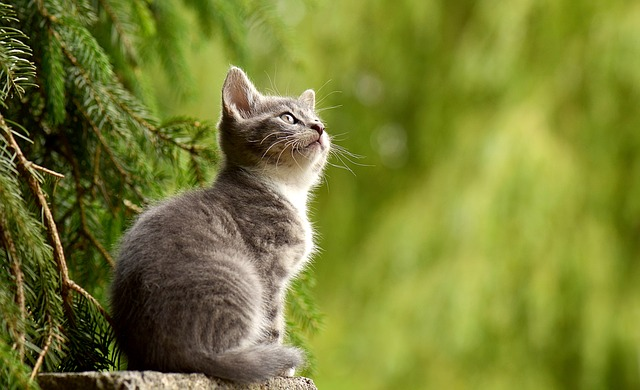
\includegraphics[width=\linewidth]{cat1}\\%
  Caption 1
  \end{minipage}%
%
  \begin{minipage}{10px}\end{minipage}
  \begin{minipage}{0.47\linewidth}%
  \centering
      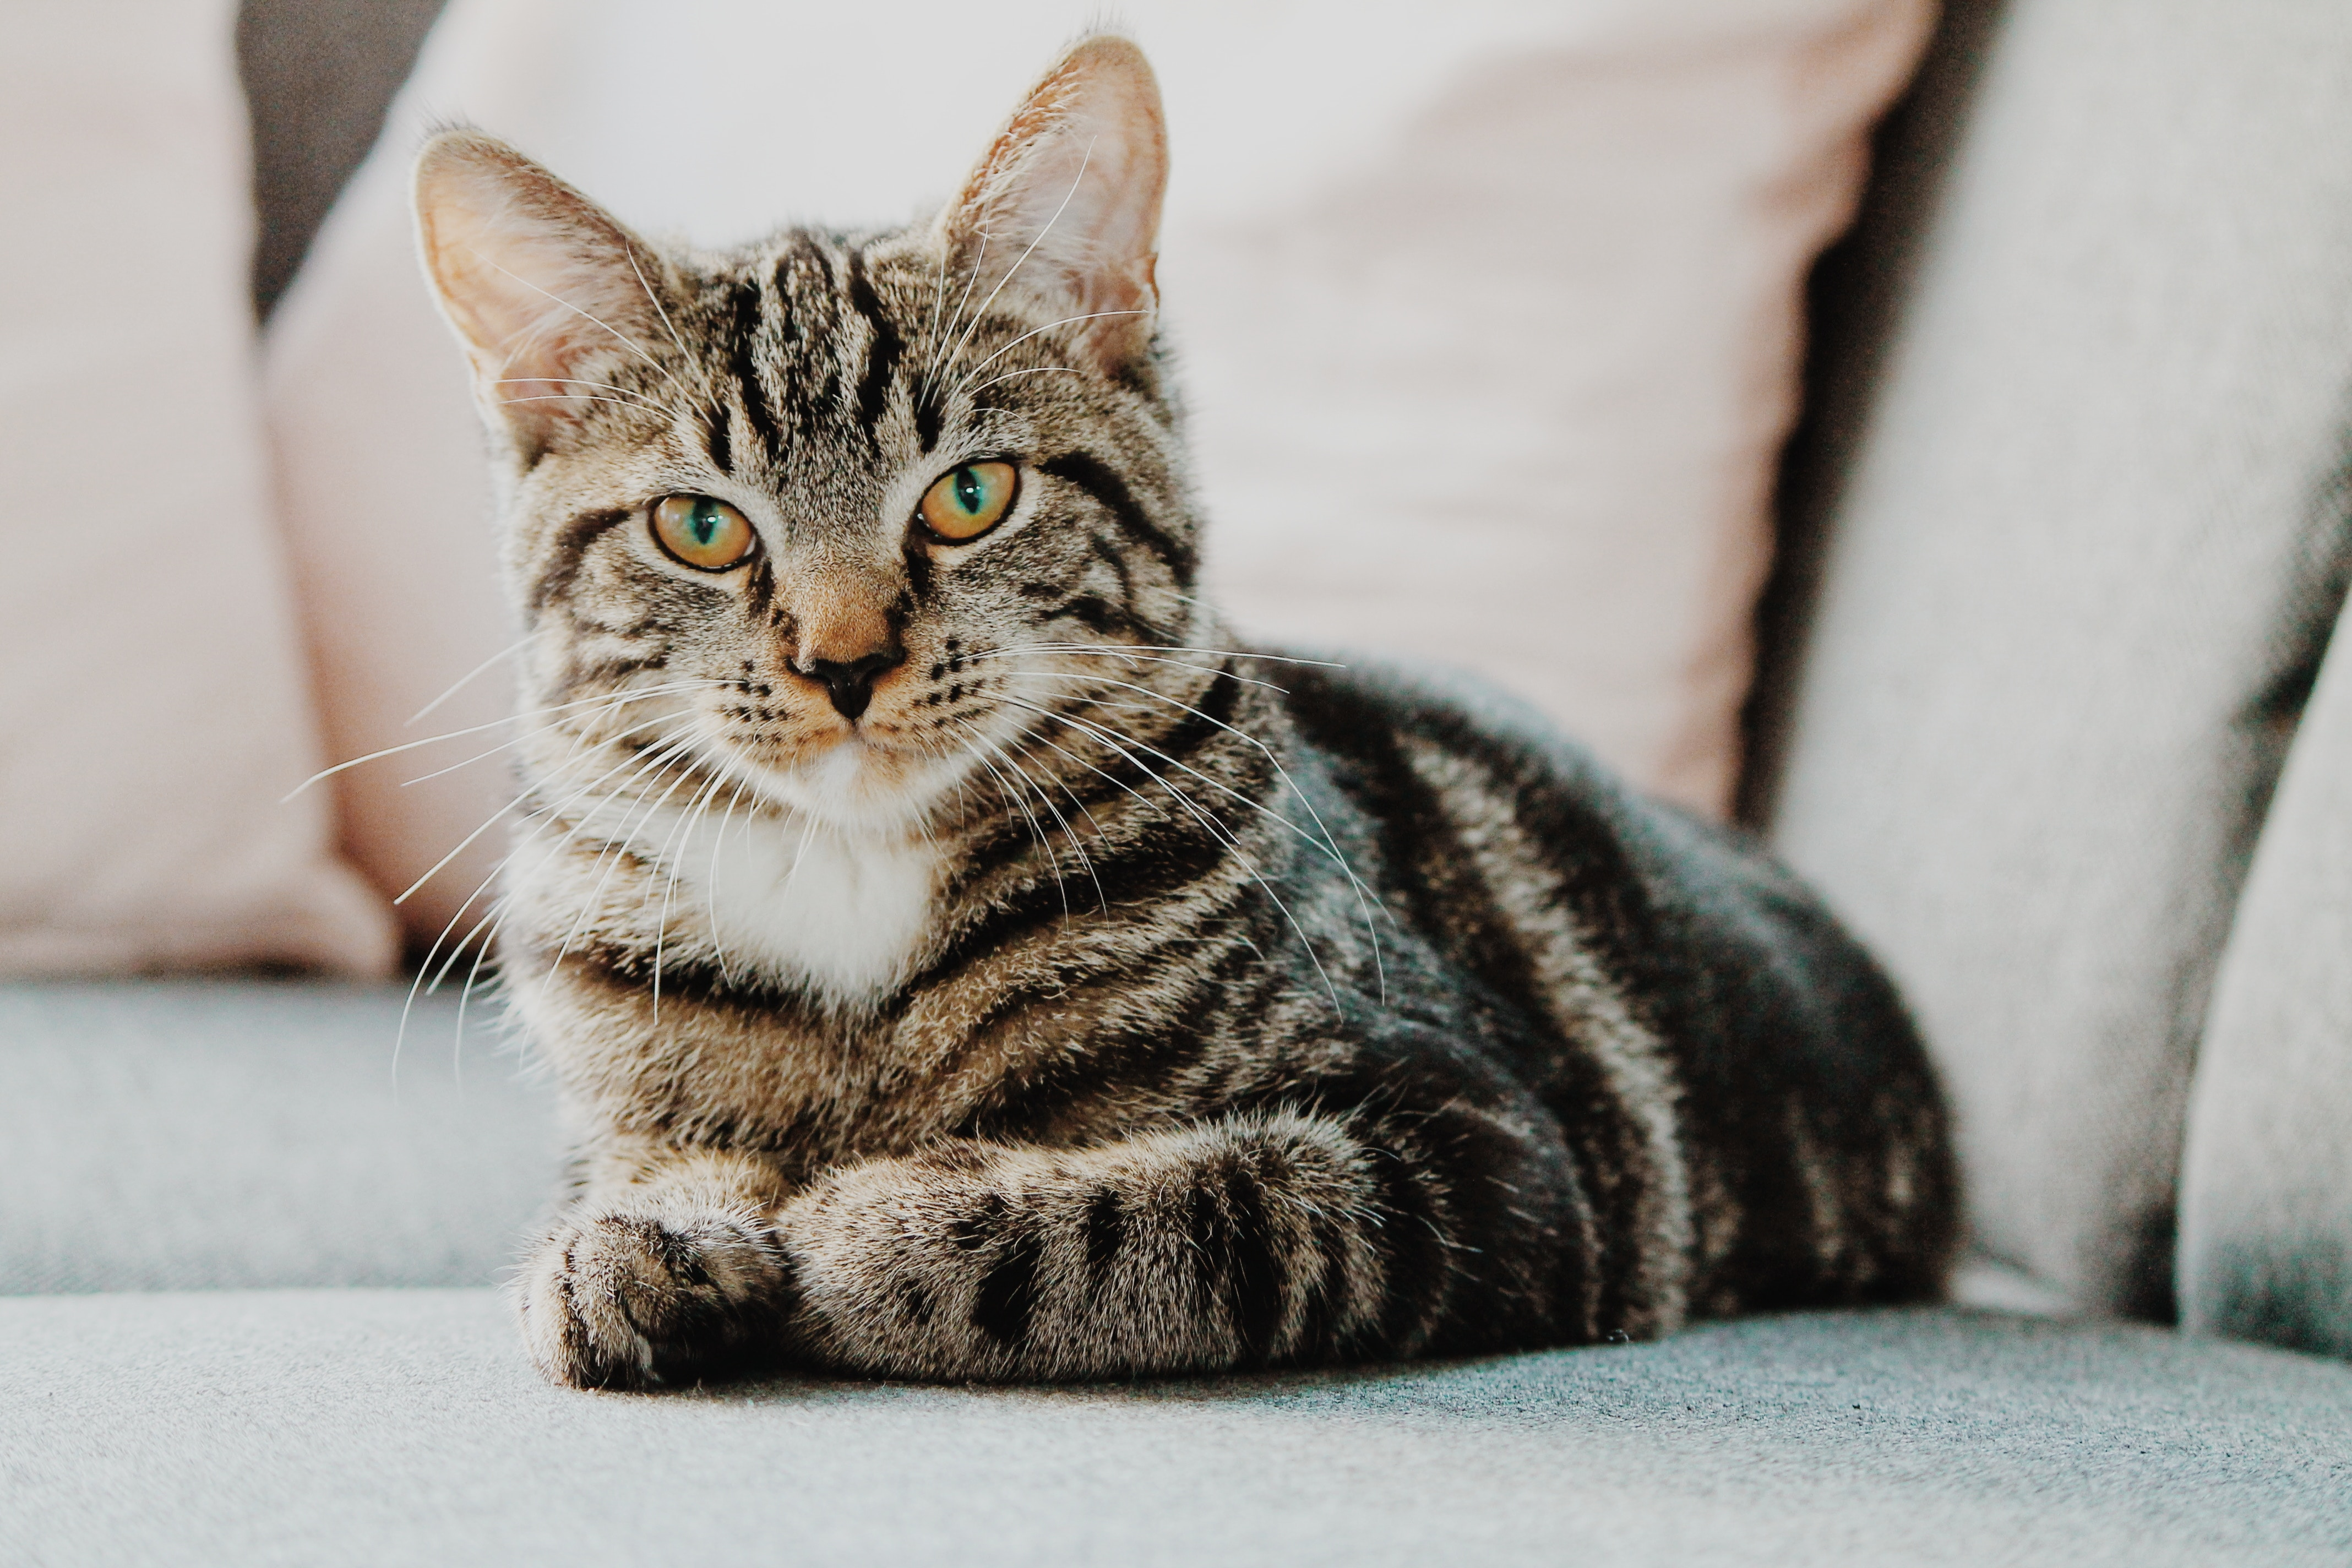
\includegraphics[width=\linewidth]{cat2}\\%
  Caption 2
  \end{minipage}%

\end{posterbox}

\begin{posterbox}[name=references, column=1, span=2, below=expe, below=intro,
                  below=name3, bottomaligned=notation]{Acknowledgement \& References}
\neutralisetitre
\bibliographystyle{plain}
% smaller text:
{\small\setstretch{0.9}
This work was funded by ...

\begin{thebibliography}{1}

\bibitem{ElGhaoui_Viallon_Rabbani12}
L.~{El Ghaoui}, V.~Viallon, and T.~Rabbani.
\newblock Safe feature elimination in sparse supervised learning.
\newblock {\em J. Pacific Optim.}, 8(4):667--698, 2012.
\\[-0.5cm]

\end{thebibliography}
}
\end{posterbox}

\end{poster}
\end{document}
